% 4_results.tex
\section{Results}
\label{sec:results}

All accuracies are balanced accuracy in the per-sightline normalization regime,
summarized as the p16 of $\nseedfold$ seed-fold values unless noted. The numbers
of record are the dedicated-binary measurements; they supersede earlier
multiclass sub-block estimates.

\subsection{Distinguishability lattice and strong-AGN detection}
\label{sec:results:lattice}

Table~\ref{tab:lattice} reports the pairwise lattice at $M=64$.
\latClearedTotal{} of the \latClearedTotal{} recipe pairs not involving the
stellar-wind/wind${+}$AGN comparison clear the $\latQualBar$ separability floor on
the p16 edge: no-feedback versus stellar wind at $\latCaCb$, no-feedback versus
wind${+}$AGN at $\latCaCc$, no-feedback versus wind${+}$strong-AGN at $\latCaCd$,
stellar-wind versus wind${+}$strong-AGN at $\latCbCd$, and wind${+}$AGN versus
wind${+}$strong-AGN at $\latCcCd$. The strong-AGN recipe is detectable against
the other three pooled at $\latCdRest$, clearing the $\detQualBar$ detection bar.
The single pair that does not clear the floor at $M=64$ is stellar wind versus
wind${+}$AGN at $\latCbCc$, near chance; this pair is the subject of
Section~\ref{sec:results:weak}.

\begin{table}
  \centering
  \caption{Pairwise distinguishability lattice at stacking depth $M=64$,
    per-sightline regime, dedicated binary classifier, balanced accuracy p16
    (16th percentile of $\nseedfold$ seed-fold values). Verdict is PASS if p16
    $\geq\latQualBar$ (pairs) or $\geq\detQualBar$ (detection cell). The
    stellar-wind/wind${+}$AGN pair (C2--C3) does not clear at $M=64$ and is
    deferred to Section~\ref{sec:results:weak}. Source:
    \texttt{results/reframe\_suite/hardening/pair\_binary\_summary.csv}.}
  \label{tab:lattice}
  \begin{tabular}{llc}
    \hline
    Pair & p16 (bal.\ acc.) & Verdict \\
    \hline
    C1--C2 (NoFB vs StellarWind)        & \latCaCb & PASS \\
    C1--C3 (NoFB vs WindAGN)            & \latCaCc & PASS \\
    C1--C4 (NoFB vs WindStrongAGN)      & \latCaCd & PASS \\
    C2--C4 (StellarWind vs WindStrongAGN) & \latCbCd & PASS \\
    C3--C4 (WindAGN vs WindStrongAGN)   & \latCcCd & PASS \\
    C2--C3 (StellarWind vs WindAGN)     & \latCbCc & deferred (\S\ref{sec:results:weak}) \\
    \hline
    C4 vs rest (detection)              & \latCdRest & PASS \\
    \hline
  \end{tabular}
\end{table}

\begin{figure}
  \centering
  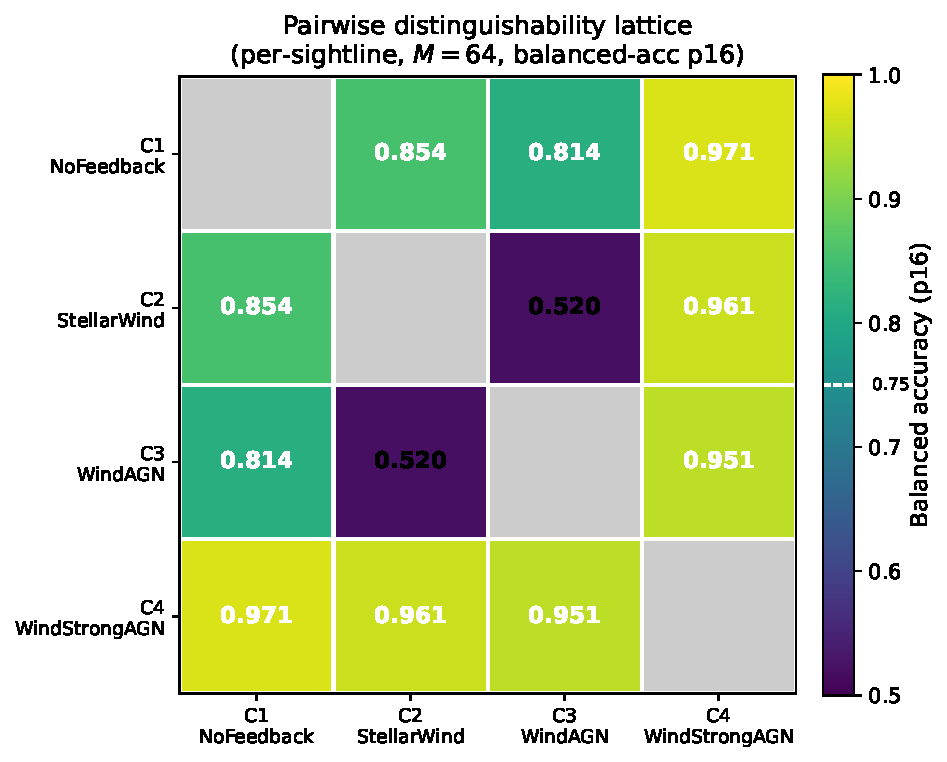
\includegraphics[width=\columnwidth]{figures/fig_lattice_M64.pdf}
  \caption{Pairwise distinguishability lattice at stacking depth $M=64$,
    per-sightline regime, dedicated binary classifier. Each off-diagonal cell is
    colored by the balanced-accuracy p16 (16th percentile of $\nseedfold$
    seed-fold values) for that recipe pair, annotated with its value; the
    diagonal is blanked. The colormap runs from chance ($0.5$, light) to unity
    (dark), with the $\latQualBar$ separability floor marked on the colorbar. All
    pairs involving wind${+}$strong-AGN (C4) and all no-feedback-versus-feedback
    pairs read dark; the stellar-wind/wind${+}$AGN cell (C2--C3) reads near chance
    ($\latCbCc$). Source:
    \texttt{results/reframe\_suite/hardening/pair\_binary\_summary.csv}.}
  \label{fig:lattice}
\end{figure}

\subsection{Stacking-depth scaling}
\label{sec:results:mscaling}

Distinguishability rises monotonically with stacking depth for every pair, which
turns each cell into a data-volume requirement. The no-feedback-versus-feedback
and strong-AGN pairs reach the $\latQualBar$ floor by $M\approx16$--$32$ and
saturate near unity by $M=256$. The 4-class context tracks this: 4-class balanced
accuracy is at chance per sightline ($\fourclassMone$ at $M=1$) and climbs to
$\fourclassMsixfour$ at $M=64$ and $\fourclassMtwofivesix$ at $M=256$ on the
lower-CI edge. The slowest-rising cell is the stellar-wind/wind${+}$AGN pair
(Section~\ref{sec:results:weak}).

\begin{figure}
  \centering
  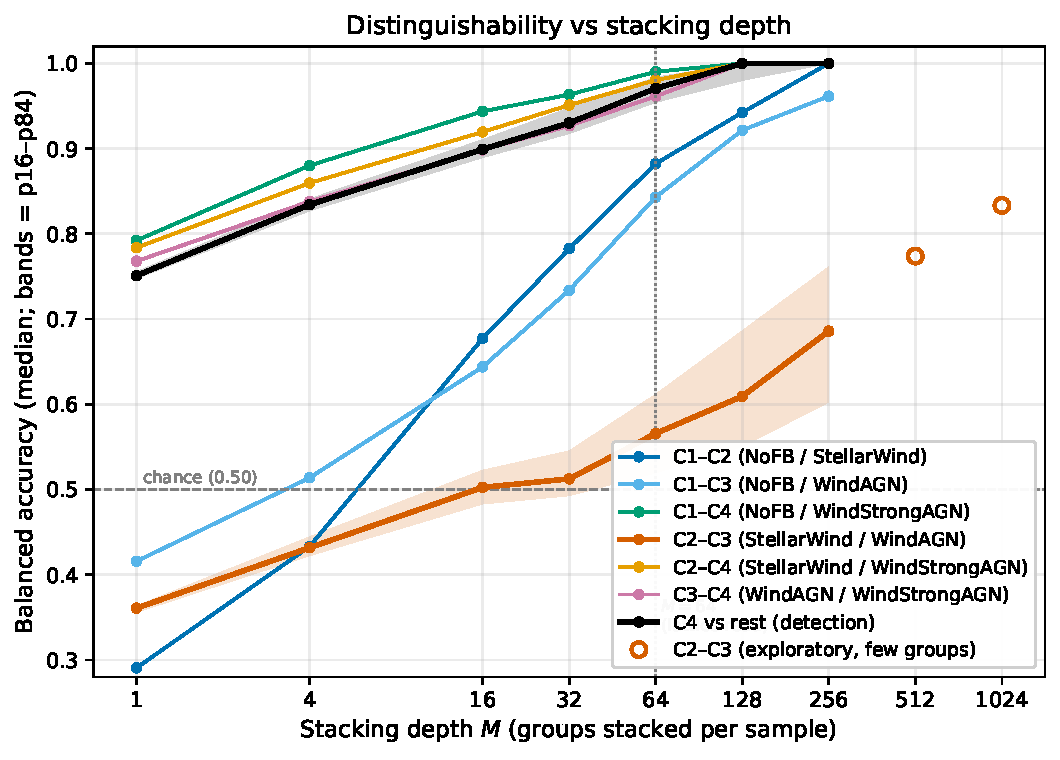
\includegraphics[width=\columnwidth]{figures/fig_acc_vs_M.pdf}
  \caption{Distinguishability versus stacking depth $M$ (log axis), per-sightline
    regime, one line per recipe pair plus the C4-versus-rest detection curve.
    Markers are the median balanced accuracy; the headline lines
    (stellar-wind/wind${+}$AGN and C4-versus-rest) carry shaded p16--p84 bands.
    The dashed horizontal line is chance ($0.5$) and the dotted vertical guide
    marks $M=64$, the lattice read point (Fig.~\ref{fig:lattice}). The
    no-feedback-versus-feedback and strong-AGN pairs saturate near unity by
    $M=256$, while the stellar-wind/wind${+}$AGN pair (vermillion) is the slow
    riser, still climbing at $M=256$; its exploratory $M=512$/$1024$ points are
    shown as hollow markers. Source:
    \texttt{results/reframe\_suite/hardening/pair\_binary\_summary.csv}.}
  \label{fig:accvsM}
\end{figure}

\subsection{Stellar-wind versus wind+AGN: a weak signal that emerges with stacking}
\label{sec:results:weak}

The stellar-wind versus wind${+}$AGN pair is indistinguishable per sightline and
near chance at $M=64$ ($\latCbCc$), but its distinguishability rises with stacking
depth: median balanced accuracy climbs from $\hbcMone$ at $M=1$ through
$\hbcMsixfour$ at $M=64$ and $\hbcMonetwoeight$ at $M=128$ to $\hbcMtwofivesix$ at
$M=256$, where the p16 reaches $\hbcMtwofivesixPsixteen$ and clears the
$\hbcGate$ routing gate. This retires the prior reading of this pair as an
intrinsic null. The signal is weak and the gate is marginal, and we state the
caveats on the face of the claim:
\begin{itemize}
  \item \textbf{Gate-marginal.} The p16 at $M=256$ is $\hbcMtwofivesixPsixteen$,
        a $\hbcGateMargin$ hug of the $\hbcGate$ line; the bootstrap probability
        that p16 clears $\hbcGate$ is $\hbcBootP$, and the $95\%$ confidence
        interval on the p16 ($[\hbcCIlo,\hbcCIhi]$) straddles $\hbcGate$.
  \item \textbf{Weak.} The pair needs $M\geq\hbcMmin$ to clearly exceed chance;
        below that it is at or near chance.
  \item \textbf{Exploratory high-$M$ extension.} Median balanced accuracy reaches
        $\hbcMfivetwelve$ at $M=512$ and $\hbcMtenfourtwentyfour$ at $M=1024$,
        but these depths have few groups and are flagged exploratory.
\end{itemize}

The three controls (Section~\ref{sec:results:controls}) are what license claiming
this weak rise as a real $P_F(k)$-shape feedback signal rather than an artifact.

\subsection{Controls}
\label{sec:results:controls}

\textbf{Self-pair null.} The within-class stellar-wind self-pair stays at chance
across stacking: $\selfpairMsixfour$ at $M=64$ and $\selfpairMtwofivesix$ at
$M=256$. By the pre-stated criterion --- a self-pair climbing above
$\selfpairCrit$ at $M=256$ would indicate a stacking-variance artifact --- the
criterion is not met, so the stellar-wind/wind${+}$AGN rise is not a finite-$M$
variance effect.

\textbf{Mean-flux baseline.} The mean-flux-only baseline for the
stellar-wind/wind${+}$AGN pair stays flat at chance at every depth
($\leq\fbarCbCcMax$), so that pair's rise is carried entirely by $P_F(k)$ shape,
not by the mean-flux offset. Across the lattice, the recipe ordering correlates
with per-class mean flux (Spearman $\hthreeSpearman$), but $P_F(k)$ carries
separability beyond mean flux at every cell when measured off the accuracy
ceiling. At the non-saturated $M=16$ read the headroom is clean and large
(strong-AGN-versus-rest $+\hthreeCdRestSixteen$, stellar-wind-versus-strong-AGN
$+\hthreeCbCdSixteen$, wind${+}$AGN-versus-strong-AGN $+\hthreeCcCdSixteen$; all
clear the $+\hthreeBar$ bar), and the no-feedback-versus-feedback cells clear by
$+\hthreeNoFBlo$ to $+\hthreeNoFBhi$ everywhere. At the saturated $M=64$ read the
strong-AGN headroom is thinner ($+\hthreeCdRestSat$, $+\hthreeCbCdSat$,
$+\hthreeCcCdSat$), because both estimators approach the accuracy ceiling. The
honest reading is that the mean-flux ordering is real and substantial, with a
real $P_F(k)$-shape residual on top of it.

\textbf{Injection-recovery sensitivity.} The $\alpha=0$ calibration centers at
chance ($\hfourAlphaZeroMsixfour$ median at $M=64$), so the instrument is valid.
The minimum detectable amplitude is $\delta_\mathrm{min}(M{=}64)=\hfourDeltaMin$:
the pipeline detects a $P_F(k)$-shape perturbation of $\hfourDeltaMinPct\%$ of the
strong-AGN-minus-stellar-wind template at $M=64$. The real
stellar-wind/wind${+}$AGN difference is nearly orthogonal to that template: its
projection has an effective amplitude $\alpha_\mathrm{equiv}\approx\hfourAlphaEquiv$
against a template scale $\beta=\hfourBeta$, so a template-aligned perturbation of
that amplitude would be undetectable. The stellar-wind/wind${+}$AGN signal is
therefore a distinct, weaker spectral signature, not a scaled-down version of the
strong-AGN signal, and the injection instrument calibrates sensitivity along the
strong-AGN template direction only; the stellar-wind/wind${+}$AGN claim rests on
the self-pair and mean-flux controls, not on this instrument.

\begin{figure}
  \centering
  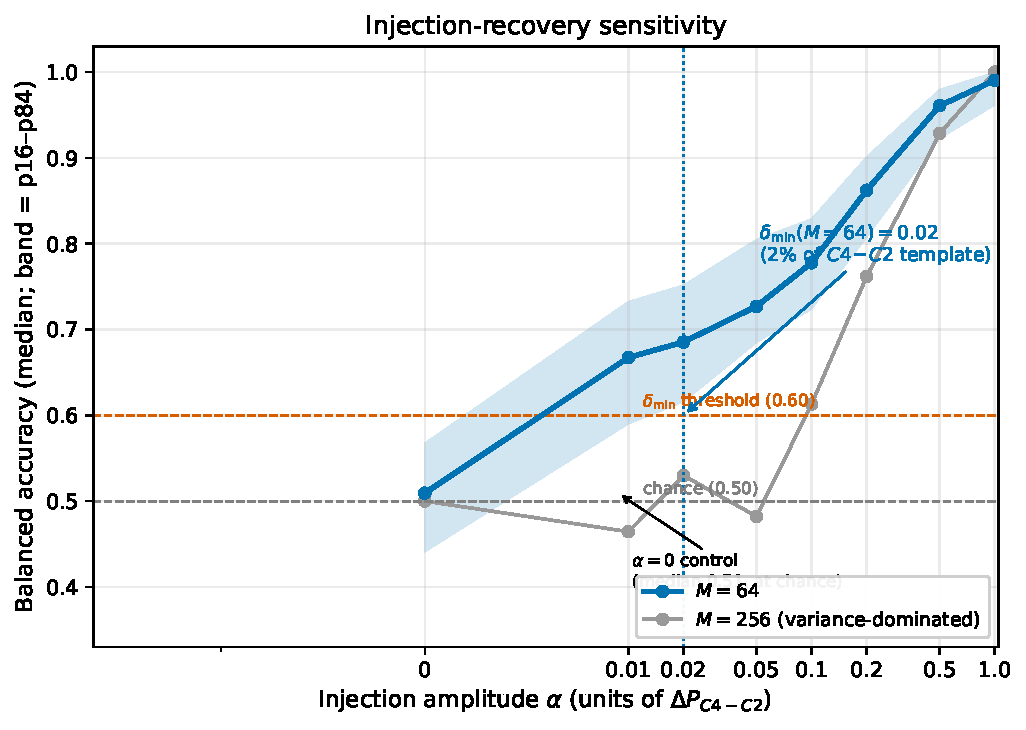
\includegraphics[width=\columnwidth]{figures/fig_injection_sensitivity.pdf}
  \caption{Injection-recovery sensitivity: balanced accuracy versus injection
    amplitude $\alpha$ (in units of the strong-AGN-minus-stellar-wind template
    $\Delta P_{C4-C2}$). The solid line is $M=64$ with a shaded p16--p84 band; the
    fainter line is $M=256$, which is variance-dominated at low $\alpha$. The
    $\alpha=0$ control sits at chance (median $\hfourAlphaZeroMsixfour$ at $M=64$),
    confirming the instrument is calibrated. Dashed lines mark chance ($0.5$) and
    the $0.60$ detection threshold; the minimum detectable amplitude
    $\delta_\mathrm{min}(M{=}64)=\hfourDeltaMin$ is where the $M=64$ p16 first
    reaches $0.60$, i.e. a $P_F(k)$-shape perturbation of $\hfourDeltaMinPct\%$ of
    the strong-AGN-minus-stellar-wind template. Source:
    \texttt{results/reframe\_suite/hardening/injection\_recovery\_summary.csv}.}
  \label{fig:injection}
\end{figure}

\subsection{Non-claims}
\label{sec:results:nonclaims}

We state the binding scope limits verbatim. We do not claim per-sightline
feedback identification at $z\approx\zsnap$ from $P_F(k)$ alone. The stacking move
($M$ up to $256$) materially changes the problem from single-sightline inference
to within-class population statistics. The lower-CI accuracies reported here are
operational internal gates, not externally-defensible classification benchmarks.
All lattice and detection numbers are conditional on fixed cosmology, ultraviolet
background, and thermal history within one Sherwood realization; no nuisance
marginalization was performed.
